\documentclass[12pt]{article}
\usepackage{amsmath, amssymb}
\usepackage{graphicx}
\usepackage{caption}
\usepackage{geometry}
\geometry{margin=1in}

\title{Prime Numbers Distribution in 6D via Dimensionality Reduction}
\author{Shaimaa Said Soltan}
\date{}

\begin{document}

\maketitle

\section*{Abstract}
This document presents the dimensionality reduction concept used to visualize 
prime number distribution in a 6-dimensional structure projected into 2D. 
The method uses two prime branches and a coprime–product sieve to count 
distinct composites and derive the prime count formula.

\section{Dimensionality Reduction Concept}

The following figure illustrates the 6-side (hexahedral) structure used to 
represent prime number distribution in higher dimensions.

\begin{figure}[h!]
    \centering
    % Replace placeholder with your actual file name
    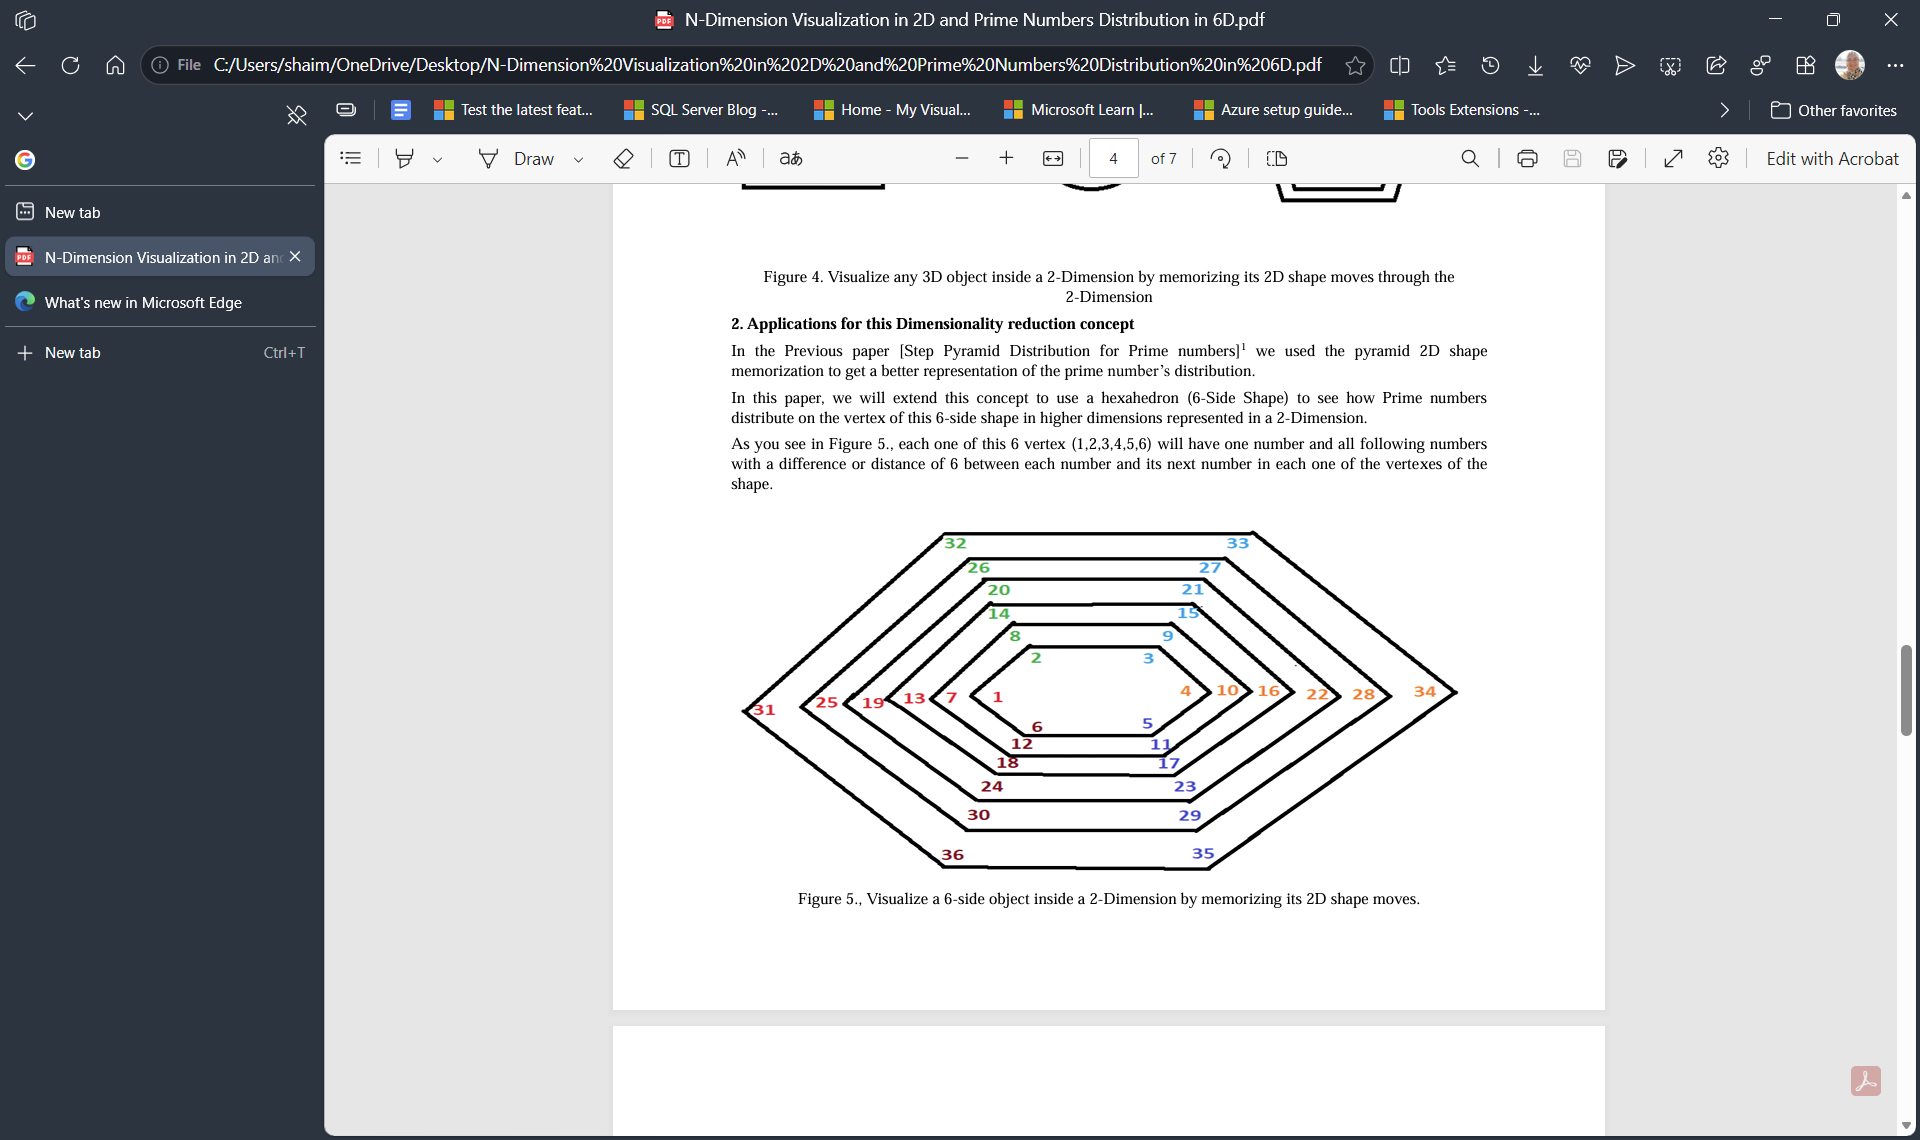
\includegraphics[width=0.85\textwidth]{image_hexagon_placeholder.png}
    \caption{Visualization of a 6-side object inside 2D (Figure 5).}
\end{figure}

Each vertex of the 6-side shape contains numbers spaced by 6, forming 
six infinite arithmetic branches. Two of these branches contain all primes 
greater than 3:



\[
\text{Branch 1} = \{1, 7, 13, 19, 25, 31, \dots\}
\]




\[
\text{Branch 5} = \{5, 11, 17, 23, 29, 35, \dots\}
\]



If the shape is extended to size \(6V\), each branch contains \(V\) numbers, 
and the two prime branches contain:



\[
2V - 1
\]



candidate positions.

\section{Coprime–Product Matrix}

The coprime–product matrix is constructed using \(m\) prime pairs. 
The matrix detects composite numbers by generating all coprime products 
across the two branches.

Below are placeholders for the two matrix images:

\begin{figure}[h!]
    \centering
    % Replace placeholder with your actual file name
    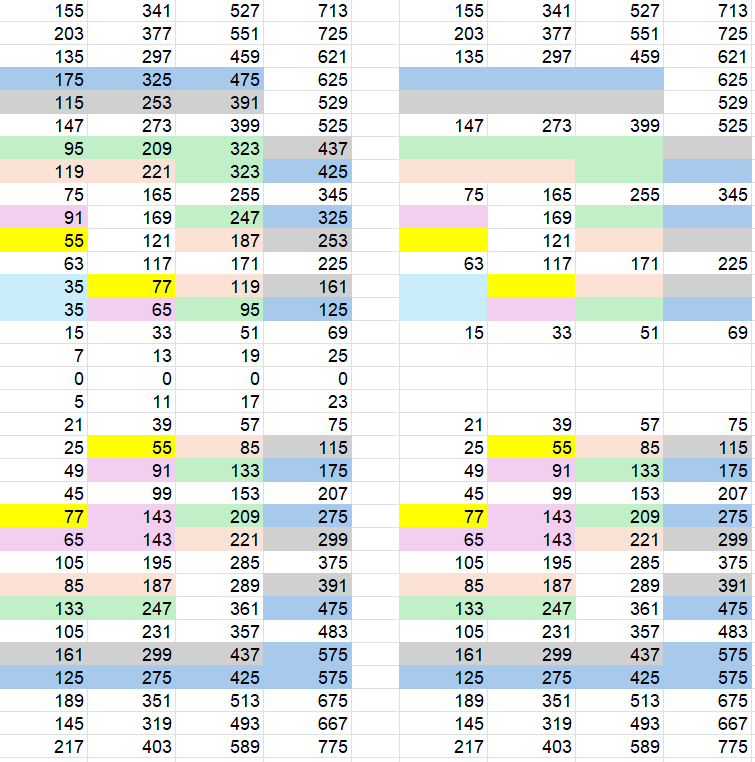
\includegraphics[width=0.85\textwidth]{image_matrix_left_placeholder.png}
    \caption{Left coprime–product matrix (distinct composite detection).}
\end{figure}

\begin{figure}[h!]
    \centering
    % Replace placeholder with your actual file name
    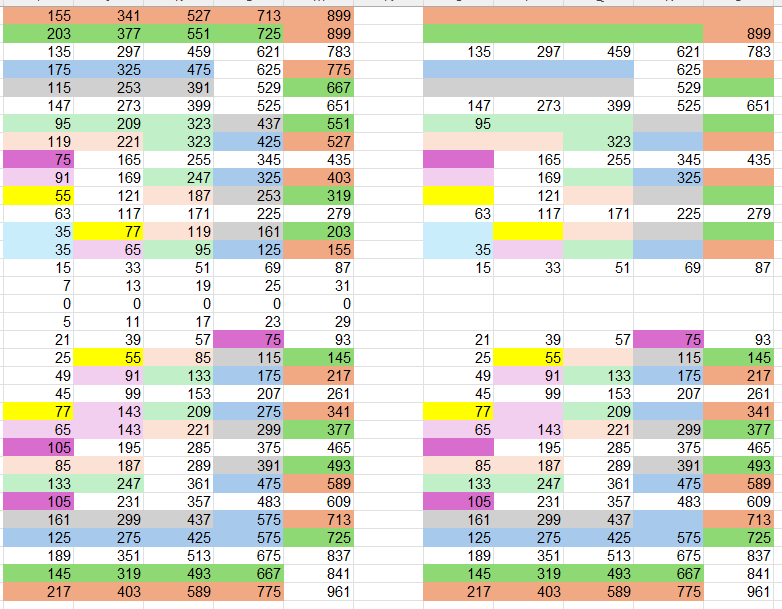
\includegraphics[width=0.85\textwidth]{image_matrix_right_placeholder.png}
    \caption{Right coprime–product matrix (mirrored structure).}
\end{figure}

\section{Distinct Coprime Count}

The number of distinct coprime composites detected by the sieve is:



\[
C_{\text{distinct}}
=
m(N-1)
-
\sum_{i=1}^{2m-1} i
\]



Using the triangular number identity:



\[
\sum_{i=1}^{2m-1} i
=
\frac{(2m-1)(2m)}{2}
\]



Thus the closed form becomes:



\[
C_{\text{distinct}}
=
m(N-1)
-
\frac{(2m-1)(2m)}{2}
\]



\section{Prime Count Formula}

Since the two prime branches contain \(2V - 1\) candidates, and the sieve 
detects all composites, the number of primes is:



\[
\text{PrimeCount}
=
(2V - 1)
-
C_{\text{distinct}}
\]



Substituting:



\[
\text{PrimeCount}
=
(2V - 1)
-
\left[
m(N-1)
-
\frac{(2m-1)(2m)}{2}
\right]
\]



\section{Variable Definitions}



\[
\begin{aligned}
m &= \text{number of prime pairs (columns in the coprime matrix)} \\
N &= \text{maximum index used in the coprime matrix} \\
V &= \text{length of each prime branch in the 6-side structure} \\
C_{\text{distinct}} &= \text{distinct coprime composites detected} \\
\text{PrimeCount} &= \text{number of primes in the two branches}
\end{aligned}
\]



\end{document}
